\documentclass[11pt, fleqn]{article}

\usepackage[usenames,dvipsnames,svgnames,table]{xcolor}
\usepackage{amsmath}
\usepackage{amsfonts}
\usepackage[margin=1in]{geometry} % To set the margin widths
\usepackage{graphicx}
\usepackage{listings}
\usepackage{multirow}
\usepackage{tabularx}
\usepackage{varioref}
\usepackage[noabbrev,capitalize]{cleveref}
\usepackage[group-separator={,}]{siunitx}
\usepackage{subcaption}
\usepackage{titlesec}
\usepackage{lscape}
\usepackage{bm}
\usepackage[titletoc,toc,title]{appendix}

\lstset{
  frame=single,
  basicstyle=\ttfamily,% print whole listing small
  language=R,
  aboveskip=3mm,
  belowskip=3mm,
  showstringspaces=false,
  columns=flexible,
  numbers=none,
  commentstyle=\color{ForestGreen},
  stringstyle=\color{Maroon},
  breaklines=true,
  breakatwhitespace=true,
  tabsize=2,
  literate={<-}{{$\gets$}}1 {~}{{$\sim$}}1
}

\sisetup{output-exponent-marker=\textsc{e}}

\setlength{\parskip}{12pt} % Sets a blank line in between paragraphs
\setlength\parindent{0pt} % Sets the indent for each paragraph to zero

\begin{document}

\title{Machine Learning (41204-01)\\HW \#5}
\author{Will Clark $\vert$ Matthew DeLio \\
\texttt{\{will.clark,mdelio\}@chicagobooth.edu} \\
University of Chicago Booth School of Business}
\date{\today}
\maketitle

\section{Baseline Predictive Models} \label{baseline}

We use a multinomial logistic regression, a random forest, and a boosting tree as a set of baseline models/algorithms against which we can assess the performance of the neural networks discussed in \vref{sec:nnets}. 

First, we use a multinomial logistic regression model with an L1 penalty for variable selection/reduction. We use five-fold cross validation to select the optimal regularization parameter for each classification (i.e. there are six logistic regression models, each with its own L1 penalty). On our test data set, we find that this model predicts movement type with 95.4\% accuracy. We can see in \vref{fig:heatmap_dmr,tab:conmat_dmr} that the model predicts extremely well overall. The most common mistake it makes is to confuse standing/sitting, and it sometimes has trouble distinguishing between walking vs. walking up or down stairs.\footnote{We find the heatmap representation of the confusion matrix to be a quick and helpful way to visualise a model's predictive accuracy. Full tabular results can be found in the appendix.}

Next, we try a random forest algorithm. The only parameter to tune for a random forest is the number of covariates sampled at each tree split (\texttt{mtry}). A rule of thumb is to set $\texttt{mtry}=\sqrt{p}$. In this case, $p=477$, so we estimated a random forest for each of $\texttt{mtry}\in(10, 15, 20, 25, 30)$ so that the range would be roughly centered around $\sqrt{p}$. Again using five-fold cross validation, we found the optimal \texttt{mtry} to be 10. This model predicts out of sample with 94.0\% accuracy, making it slightly less effective than our multinomial logit model above.\footnote{In sample accuracy was above 98\%, although the training and test set are composed of different groups of people, so we should not be surprised to see lower OOS accuracy.} We can see in \vref{fig:heatmap_rf,tab:conmat_rf} that this algorithm, like the one discussed above, also confuses sitting and standing. It also tends to get a bit more confused between walking vs. walking up/down stairs than the multinomial logit model.

Lastly, we try a boosting tree algorithm. The parameters we can use to tune and the ranges over which we sampled are:
\begin{itemize}
\item \texttt{interaction.depth} $\in (1, 5, 9)$
\item \texttt{n.trees} $\in (500, 1000, 1500, 2000)$
\item \texttt{shrinkage} $\in (0.01, 0.05)$
\end{itemize}
The optimal algorithm, again chosen by five-fold cross validation, used 2000 trees, interaction depth of 5, and a shrinkage parameter of 0.05. This algorithm predicts out of sample with 94.4\% accuracy, making it slightly more accurate than the random forest but still not as accurate as our multinomial logit model. We can see in \vref{fig:heatmap_boost,tab:conmat_boost} that this algorithm is worse than the two prior at distinguishing between sitting/standing, but it does slightly better than the random forest at distinguishing between walking vs. walking on stairs.

\section{Neural Nets} \label{sec:nnets}
To begin our investigation of using neural networks we started fairly modestly with a hyperbolic tangent activation, with 2-hidden layers containing 200 nodes each, trained over 10 epochs.  With these settings, the out-of-sample accuracy was a modest 92.6\%.  To improve on this, we decided to keep the number of hidden layers at 2, but to tweak the number of nodes in each hidden layer to be: $\dim input + \dim classifiers = 477 + 6 = 483$.  With these hidden layers set we then tried the following activations:
\begin{itemize}
\item TanH
\item TanH with Dropout
\item Rectifier With Dropout
\end{itemize}

We found that the Rectifier with Dropout seemed to perform the best and then further tweaked the hidden dropout ratio, input dropout ratio, and added l1/l2 penalties (l2 penalties seemed to hurt accuracy, so they were removed).  With accuracy standing at 93.2\%, with just 10 epochs, we then decided to turn up the number of epochs to 500 (see \cref{lst:neural} for final settings).  Running the extra epochs further increased out-of-sample accuracy to 94.6\%.

\Cref{tab:overall} shows a crude comparison of the overall accuracy by model type.  The neural network fairs pretty well overall, inferior only to the multinomial regression in terms of raw accuracy.  Looking more closely at the types of class errors it makes we see that, compared to the other models, it does mistake sitting for laying more often than the other algorithms, but otherwise does a fairly decent job predicting the activity.  Finally, when compared to the other tree-based supervised learning algorithms, the neural network trains faster and is easier to tune.

\begin{table}[ht]
\centering
\caption{Overall Accuracy by Model Type}
\label{tab:overall}
\begin{tabular}{l|r}
 \hline
 \textbf{Model} & \textbf{Accuracy} \\
 \hline
 Multinomial Logit & 95.4\% \\
 Random Forest & 94.0\% \\
 Boosting Tree & 94.4\% \\
 \hline
 Neural Network & 94.6\% \\
 \hline
\end{tabular}
\end{table}

\begin{lstlisting}[float,label=lst:neural,caption=Final Deep Learning Configuration, language=R]
model.nn1 <- h2o.deeplearning(
  x = 1:p, y = p+1, 
  training_frame = h2o.cbind(dat.h2o$X_train, dat.h2o$y_train),
  activation = "RectifierWithDropout",
  input_dropout_ratio = 0.50,
  hidden = c(p+y.nlevels, p+y.nlevels),
  hidden_dropout_ratios = c(0.5, 0.5),
  epochs = 500,
  l1 = 1e-5,
  model_id = "model.nn1")
\end{lstlisting}

% latex table generated in R 3.2.1 by xtable 1.7-4 package
% Thu Nov  5 17:15:31 2015
\begin{table}[ht]
\centering
\caption{Confusion Matrix for Neural Network} 
\label{tab:conmat_nn1}
\begin{tabular}{l|rrrrrr}
  &\multicolumn{6}{c}{Reference}\\
 \hline
Predicted & Walking & WalkingUpstairs & WalkingDownstairs & Sitting & Standing & Laying \\ 
  \hline
Walking & 485 &   4 &   3 &   0 &   0 &   0 \\ 
  WalkingUpstairs &   6 & 446 &  23 &   1 &   0 &   0 \\ 
  WalkingDownstairs &   5 &  21 & 394 &   0 &   0 &   0 \\ 
  Sitting &   0 &   0 &   0 & 420 &  26 &   0 \\ 
  Standing &   0 &   0 &   0 &  53 & 506 &   0 \\ 
  Laying &   0 &   0 &   0 &  17 &   0 & 537 \\ 
   \hline
\end{tabular}
\end{table}

% latex table generated in R 3.2.1 by xtable 1.7-4 package
% Thu Nov  5 17:15:31 2015
\begin{table}[ht]
\centering
\caption{Model Statistics for Neural Network} 
\label{tab:conmat_stats_nn1}
\begin{tabular}{rrrr}
  \hline
 & Sensitivity & Specificity & Balanced Accuracy \\ 
  \hline
Class: Walking & 0.978 & 0.997 & 0.987 \\ 
  Class: WalkingUpstairs & 0.947 & 0.988 & 0.967 \\ 
  Class: WalkingDownstairs & 0.938 & 0.990 & 0.964 \\ 
  Class: Sitting & 0.855 & 0.989 & 0.922 \\ 
  Class: Standing & 0.951 & 0.978 & 0.965 \\ 
  Class: Laying & 1.000 & 0.993 & 0.996 \\ 
   \hline
\end{tabular}
\end{table}


\begin{figure}[!htb]
  \centering
  \caption{Confusion Matrix Heatmap for Neural Network}
  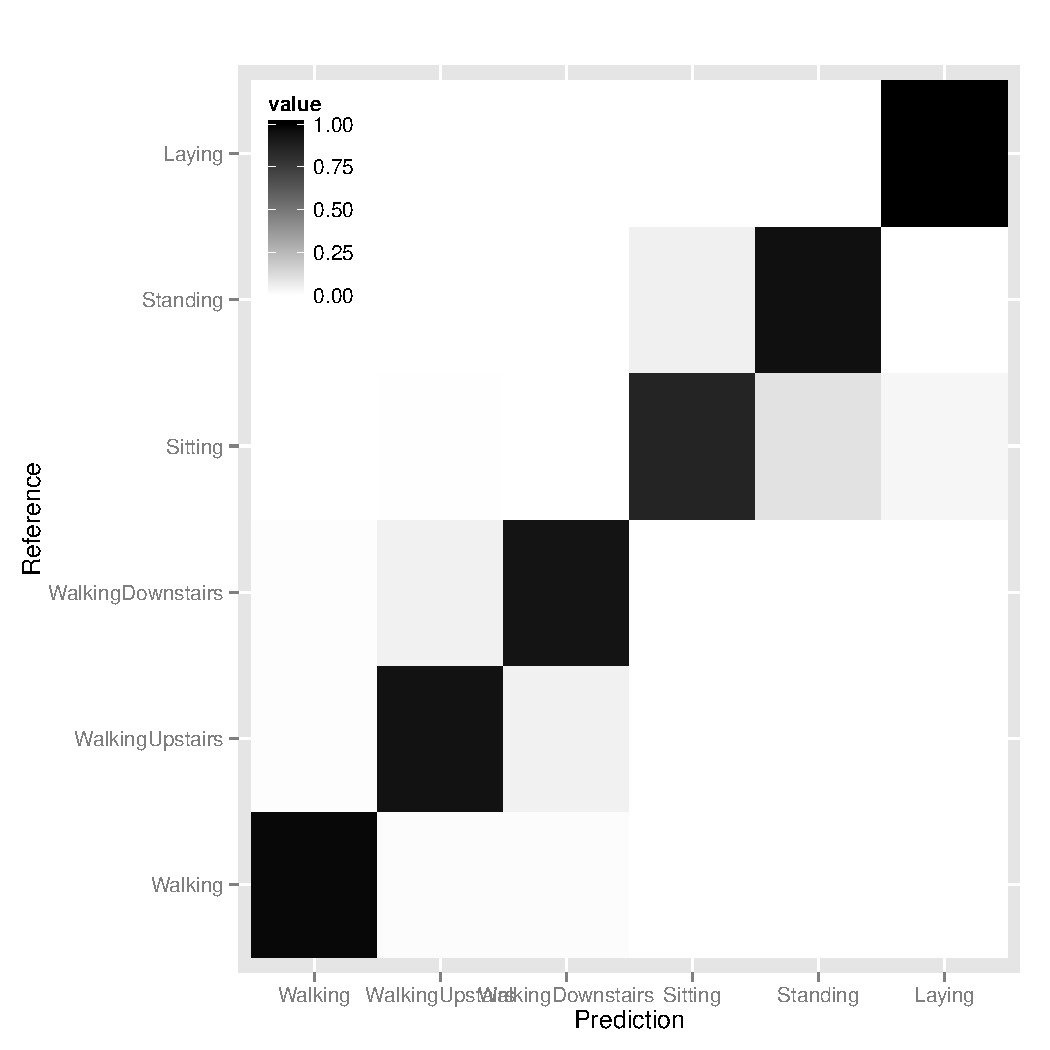
\includegraphics[scale=.5]{heatmap_nn1.pdf}
  \label{fig:heatmap_nn1}
\end{figure}

\clearpage
\begin{appendices}

\section{Confusion Heatmaps for Baseline Models}

\begin{landscape}
\begin{figure}
  \centering
  \begin{subfigure}[b]{0.45\textwidth}
    \caption{Multinomial Logit}
    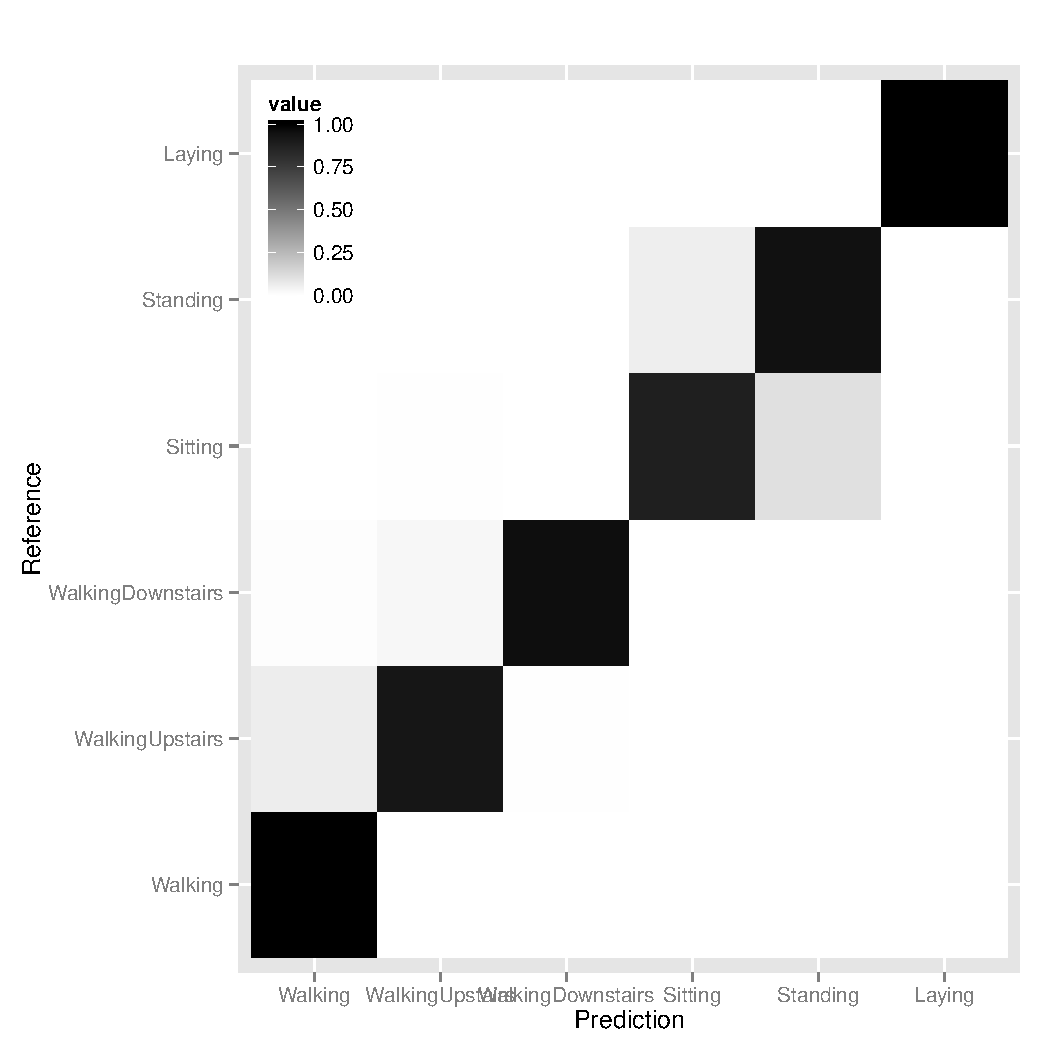
\includegraphics[width=\textwidth]{heatmap_dmr.pdf}
    \label{fig:heatmap_dmr}
  \end{subfigure}
  %\hfill
  \begin{subfigure}[b]{0.45\textwidth}
    \caption{Random Forest}
    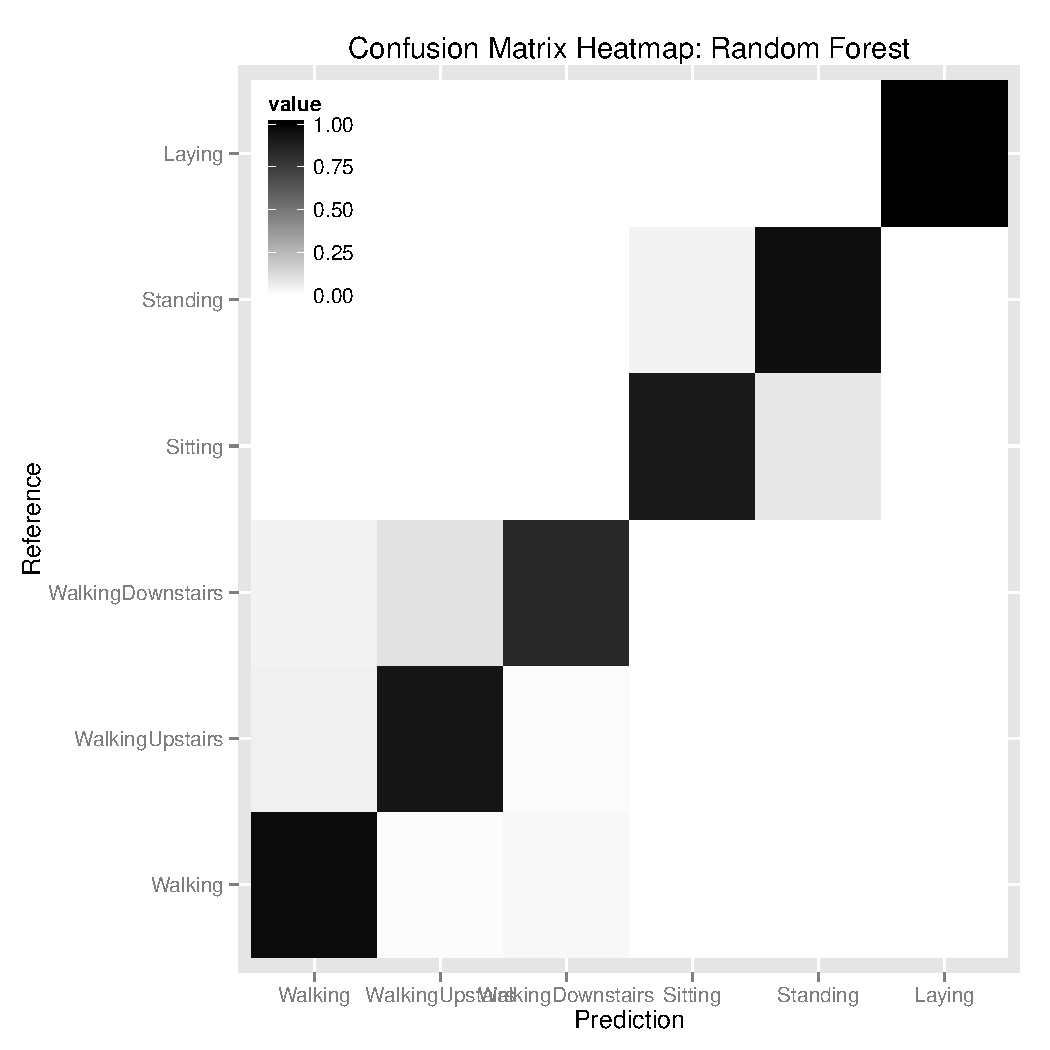
\includegraphics[width=\textwidth]{heatmap_rf.pdf}
    \label{fig:heatmap_rf}
  \end{subfigure}
  %\hfill
  \begin{subfigure}[b]{0.45\textwidth}
    \caption{Boosting Tree}
    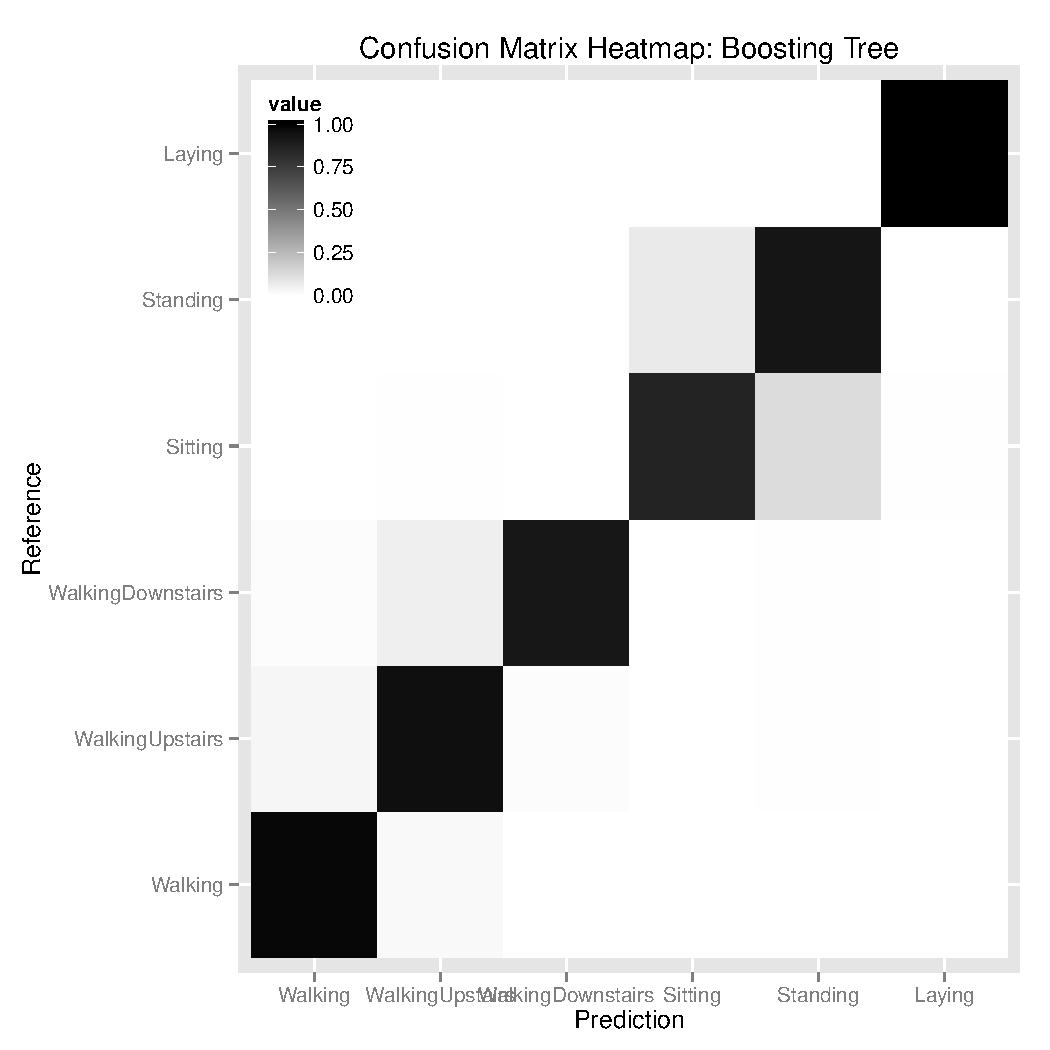
\includegraphics[width=\textwidth]{heatmap_boost.pdf}
    \label{fig:heatmap_boost}
  \end{subfigure}
  \caption{Confusion Matrix Heatmaps for Baseline Predictive Models}
\end{figure}
\end{landscape}

\section{Confusion Matrices for Baseline Models}

% latex table generated in R 3.2.2 by xtable 1.7-4 package
% Wed Nov  4 17:21:32 2015
\begin{table}[ht]
\centering
\caption{Confusion Matrix for Multinomial Logit Regression} 
\label{tab:conmat_dmr}
\begin{tabular}{rrrr}
  \hline
 & Sensitivity & Specificity & Balanced Accuracy \\ 
  \hline
Class: Walking & 1.00 & 0.99 & 0.99 \\ 
  Class: WalkingUpstairs & 0.93 & 0.99 & 0.96 \\ 
  Class: WalkingDownstairs & 0.96 & 1.00 & 0.98 \\ 
  Class: Sitting & 0.88 & 0.99 & 0.93 \\ 
  Class: Standing & 0.95 & 0.98 & 0.96 \\ 
  Class: Laying & 1.00 & 1.00 & 1.00 \\ 
   \hline
\end{tabular}
\end{table}

% latex table generated in R 3.2.2 by xtable 1.7-4 package
% Wed Nov  4 17:29:26 2015
\begin{table}[ht]
\centering
\caption{Model Statistics for Multinomial Logit Regression} 
\label{tab:conmat_stats_dmr}
\begin{tabular}{rrrr}
  \hline
 & Sensitivity & Specificity & Balanced Accuracy \\ 
  \hline
Class: Walking & 1.00 & 0.99 & 0.99 \\ 
  Class: WalkingUpstairs & 0.93 & 0.99 & 0.96 \\ 
  Class: WalkingDownstairs & 0.96 & 1.00 & 0.98 \\ 
  Class: Sitting & 0.88 & 0.99 & 0.93 \\ 
  Class: Standing & 0.95 & 0.98 & 0.96 \\ 
  Class: Laying & 1.00 & 1.00 & 1.00 \\ 
   \hline
\end{tabular}
\end{table}


% latex table generated in R 3.2.2 by xtable 1.7-4 package
% Wed Nov  4 19:31:53 2015
\begin{table}[ht]
\begin{adjustwidth}{-1in}{-1in}
\centering
\caption{Confusion Matrix for Random Forest} 
\label{tab:conmat_rf}
\begin{tabular}{l|rrrrrr}
  &\multicolumn{6}{c}{Reference}\\
 \hline
Predicted & Walking & WalkingUpstairs & WalkingDownstairs & Sitting & Standing & Laying \\ 
  \hline
Walking & 481 &  26 &  20 &   0 &   0 &   0 \\ 
  WalkingUpstairs &   5 & 439 &  47 &   0 &   0 &   0 \\ 
  WalkingDownstairs &  10 &   6 & 353 &   0 &   0 &   0 \\ 
  Sitting &   0 &   0 &   0 & 447 &  20 &   0 \\ 
  Standing &   0 &   0 &   0 &  44 & 512 &   0 \\ 
  Laying &   0 &   0 &   0 &   0 &   0 & 537 \\ 
   \hline
\end{tabular}
\end{adjustwidth}
\end{table}

% latex table generated in R 3.2.2 by xtable 1.7-4 package
% Wed Nov  4 19:31:53 2015
\begin{table}[ht]
\centering
\caption{Model Statistics for Random Forest} 
\label{tab:conmat_stats_rf}
\begin{tabular}{rrrr}
  \hline
 & Sensitivity & Specificity & Balanced Accuracy \\ 
  \hline
Class: Walking & 0.97 & 0.98 & 0.98 \\ 
  Class: WalkingUpstairs & 0.93 & 0.98 & 0.96 \\ 
  Class: WalkingDownstairs & 0.84 & 0.99 & 0.92 \\ 
  Class: Sitting & 0.91 & 0.99 & 0.95 \\ 
  Class: Standing & 0.96 & 0.98 & 0.97 \\ 
  Class: Laying & 1.00 & 1.00 & 1.00 \\ 
   \hline
\end{tabular}
\end{table}


% latex table generated in R 3.2.2 by xtable 1.7-4 package
% Wed Nov  4 19:31:53 2015
\begin{table}[ht]
\centering
\caption{Confusion Matrix for Boosting Tree} 
\label{tab:conmat_boost}
\begin{tabular}{l|rrrrrr}
  &\multicolumn{6}{c}{Reference}\\
 \hline
Predicted & Walking & WalkingUpstairs & WalkingDownstairs & Sitting & Standing & Laying \\ 
  \hline
Walking & 496 &  32 &   4 &   0 &   0 &   0 \\ 
  WalkingUpstairs &   0 & 437 &  12 &   2 &   0 &   0 \\ 
  WalkingDownstairs &   0 &   2 & 404 &   0 &   0 &   0 \\ 
  Sitting &   0 &   0 &   0 & 432 &  28 &   0 \\ 
  Standing &   0 &   0 &   0 &  57 & 504 &   0 \\ 
  Laying &   0 &   0 &   0 &   0 &   0 & 537 \\ 
   \hline
\end{tabular}
\end{table}

% latex table generated in R 3.2.2 by xtable 1.7-4 package
% Wed Nov  4 19:31:53 2015
\begin{table}[ht]
\centering
\caption{Model Statistics for Boosting Tree} 
\label{tab:conmat_stats_boost}
\begin{tabular}{rrrr}
  \hline
 & Sensitivity & Specificity & Balanced Accuracy \\ 
  \hline
Class: Walking & 0.98 & 0.99 & 0.99 \\ 
  Class: WalkingUpstairs & 0.96 & 0.99 & 0.97 \\ 
  Class: WalkingDownstairs & 0.92 & 1.00 & 0.96 \\ 
  Class: Sitting & 0.86 & 0.99 & 0.92 \\ 
  Class: Standing & 0.93 & 0.97 & 0.95 \\ 
  Class: Laying & 1.00 & 1.00 & 1.00 \\ 
   \hline
\end{tabular}
\end{table}


%\section{Code Listings}
%\lstinputlisting[label=lst:code, caption=Code Snippet, language=R]{../hw5.R}

\end{appendices}

\end{document}

% \input{.tex}

% \begin{figure}
%   \centering
%   \begin{subfigure}[b]{0.49\textwidth}
%     \caption{}
%     \includegraphics[width=\textwidth]{.pdf}
%     \label{fig:}
%   \end{subfigure}
%   \hfill
%   \begin{subfigure}[b]{0.49\textwidth}
%     \caption{}
%     \includegraphics[width=\textwidth]{.pdf}
%     \label{fig:}
%   \end{subfigure}
%   \caption{}
% \end{figure}

% \begin{figure}[!htb]
%   \centering
%   \caption{}
%   \includegraphics[scale=.5]{.pdf}
%   \label{fig:}
% \end{figure}

